\iffalse
This file is protected by Copyright. Please refer to the COPYRIGHT file
distributed with this source distribution.

This file is part of OpenCPI <http://www.opencpi.org>

OpenCPI is free software: you can redistribute it and/or modify it under the
terms of the GNU Lesser General Public License as published by the Free Software
Foundation, either version 3 of the License, or (at your option) any later
version.

OpenCPI is distributed in the hope that it will be useful, but WITHOUT ANY
WARRANTY; without even the implied warranty of MERCHANTABILITY or FITNESS FOR A
PARTICULAR PURPOSE. See the GNU Lesser General Public License for more details.

You should have received a copy of the GNU Lesser General Public License along
with this program. If not, see <http://www.gnu.org/licenses/>.
\fi

%----------------------------------------------------------------------------------------
% Update the docTitle and docVersion per document
%----------------------------------------------------------------------------------------
\def\docTitle{OpenCPI\\ ML605 Hardware Setup Guide}
\def\docVersion{1.4}
%----------------------------------------------------------------------------------------
\documentclass{article}
\iffalse
This file is protected by Copyright. Please refer to the COPYRIGHT file
distributed with this source distribution.

This file is part of OpenCPI <http://www.opencpi.org>

OpenCPI is free software: you can redistribute it and/or modify it under the
terms of the GNU Lesser General Public License as published by the Free Software
Foundation, either version 3 of the License, or (at your option) any later
version.

OpenCPI is distributed in the hope that it will be useful, but WITHOUT ANY
WARRANTY; without even the implied warranty of MERCHANTABILITY or FITNESS FOR A
PARTICULAR PURPOSE. See the GNU Lesser General Public License for more details.

You should have received a copy of the GNU Lesser General Public License along
with this program. If not, see <http://www.gnu.org/licenses/>.
\fi
\author{} % Force author to be blank
%----------------------------------------------------------------------------------------
% Paper size, orientation and margins
%----------------------------------------------------------------------------------------
\usepackage{geometry}
\geometry{
        letterpaper, % paper type
        portrait,    % text direction
        left=.75in,  % left margin
        top=.75in,   % top margin
        right=.75in, % right margin
        bottom=.75in % bottom margin
 }
%----------------------------------------------------------------------------------------
% Header/Footer
%----------------------------------------------------------------------------------------
\usepackage{fancyhdr} \pagestyle{fancy} % required for fancy headers
\renewcommand{\headrulewidth}{0.5pt}
\renewcommand{\footrulewidth}{0.5pt}
\rhead{\small{ANGRYVIPER Team}}
% \rfoot{\thepage}
%----------------------------------------------------------------------------------------
% Appendix packages
%----------------------------------------------------------------------------------------
\usepackage[toc,page]{appendix}
%----------------------------------------------------------------------------------------
% Defined Commands & Renamed Commands
%----------------------------------------------------------------------------------------
\renewcommand{\contentsname}{Table of Contents}
\renewcommand{\listfigurename}{List of Figures}
\renewcommand{\listtablename}{List of Tables}
%----------------------------------------------------------------------------------------
% Various packages
%----------------------------------------------------------------------------------------
\usepackage[usenames,dvipsnames]{xcolor} % for color names see https://en.wikibooks.org/wiki/LaTeX/Colors
\usepackage{hyperref}  % for linking urls and lists
\usepackage{graphicx}  % for including pictures by file
\usepackage{listings}  % for coding language styles
\usepackage{rotating}  % for sideways table
\usepackage{pifont}    % for sideways table
\usepackage{pdflscape} % for landscape view
\usepackage{subfig}
\usepackage{xstring}
\uchyph=0 % Never hyphenate acronyms like RCC (I think this overrides ANGRYVIPER above)
\renewcommand\_{\textunderscore\allowbreak} % Allow words to break/newline on underscores
%----------------------------------------------------------------------------------------
% Table packages
%----------------------------------------------------------------------------------------
\usepackage{longtable} % for long possibly multi-page tables
\usepackage{tabularx} % c=center,l=left,r=right,X=fill
% These define tabularx columns "C" and "R" to match "X" but center/right aligned
\newcolumntype{C}{>{\centering\arraybackslash}X}
\newcolumntype{R}{>{\raggedleft\arraybackslash}X}
\usepackage{float}
\floatstyle{plaintop}
\usepackage[tableposition=top]{caption}
\newcolumntype{P}[1]{>{\centering\arraybackslash}p{#1}}
\newcolumntype{M}[1]{>{\centering\arraybackslash}m{#1}}
%----------------------------------------------------------------------------------------
% Block Diagram / FSM Drawings
%----------------------------------------------------------------------------------------
\usepackage{tikz}
\usetikzlibrary{shapes,arrows,fit,positioning}
\usetikzlibrary{automata} % used for the fsm
%----------------------------------------------------------------------------------------
% Colors Used
%----------------------------------------------------------------------------------------
\usepackage{colortbl}
\definecolor{blue}{rgb}{.7,.8,.9}
\definecolor{ceruleanblue}{rgb}{0.16, 0.32, 0.75}
\definecolor{drkgreen}{rgb}{0,0.6,0}
\definecolor{deepmagenta}{rgb}{0.8, 0.0, 0.8}
\definecolor{cyan}{rgb}{0.0,0.6,0.6}
\definecolor{maroon}{rgb}{0.5,0,0}
%----------------------------------------------------------------------------------------
% VHDL Coding Language Style
% modified from: http://latex-community.org/forum/viewtopic.php?f=44&t=22076
%----------------------------------------------------------------------------------------
\lstdefinelanguage{VHDL}
{
        basicstyle=\ttfamily\footnotesize,
        columns=fullflexible,keepspaces,      % https://tex.stackexchange.com/a/46695/87531
        keywordstyle=\color{ceruleanblue},
        commentstyle=\color{drkgreen},
        morekeywords={
    library,use,all,entity,is,port,in,out,end,architecture,of,
    begin,and, signal, when, if, else, process, end,
        },
        morecomment=[l]--
}
%----------------------------------------------------------------------------------------
% XML Coding Language Style
% modified from: http://tex.stackexchange.com/questions/10255/xml-syntax-highlighting
%----------------------------------------------------------------------------------------
\lstdefinelanguage{XML}
{
        basicstyle=\ttfamily\footnotesize,
        columns=fullflexible,keepspaces,
        morestring=[s]{"}{"},
        morecomment=[s]{!--}{--},
        commentstyle=\color{drkgreen},
        moredelim=[s][\color{black}]{>}{<},
        moredelim=[s][\color{cyan}]{\ }{=},
        stringstyle=\color{maroon},
        identifierstyle=\color{ceruleanblue}
}
%----------------------------------------------------------------------------------------
% DIFF Coding Language Style
% modified from http://tex.stackexchange.com/questions/50176/highlighting-a-diff-file
%----------------------------------------------------------------------------------------
\lstdefinelanguage{diff}
{
        basicstyle=\ttfamily\footnotesize,
        columns=fullflexible,keepspaces,
        breaklines=true,                                % wrap text
        morecomment=[f][\color{ceruleanblue}]{@@},      % group identifier
        morecomment=[f][\color{red}]-,                  % deleted lines
        morecomment=[f][\color{drkgreen}]+,             % added lines
        morecomment=[f][\color{deepmagenta}]{---},      % Diff header lines (must appear after +,-)
        morecomment=[f][\color{deepmagenta}]{+++},
}
%----------------------------------------------------------------------------------------
% Python Coding Language Style
% modified from
%----------------------------------------------------------------------------------------
\lstdefinelanguage{python}
{
        basicstyle=\ttfamily\footnotesize,
        columns=fullflexible,keepspaces,
        keywordstyle=\color{ceruleanblue},
        commentstyle=\color{drkgreen},
        stringstyle=\color{orange},
        morekeywords={
    print, if, sys, len, from, import, as, open,close, def, main, for, else, write, read, range,
        },
        comment=[l]{\#}
}
%----------------------------------------------------------------------------------------
% Fontsize Notes in order from smallest to largest
%----------------------------------------------------------------------------------------
%    \tiny
%    \scriptsize
%    \footnotesize
%    \small
%    \normalsize
%    \large
%    \Large
%    \LARGE
%    \huge
%    \Huge

\date{Version \docVersion} % Force date to be blank and override date with version
\title{\docTitle}
\lhead{ML605 Hardware Setup Guide}
%----------------------------------------------------------------------------------------
%\usepackage[T1]{fontenc} % http://tex.stackexchange.com/a/181119
\usepackage{graphicx}
\graphicspath{ {figures/} }
\usepackage{textcomp}
\newcommand{\shellcmd}[1]{\texttt{\$ #1\\}}
\begin{document}
\maketitle
%\thispagestyle{fancy}
\newpage
	\begin{center}
	\textit{\textbf{Revision History}}
		\begin{table}[H]
		\label{table:revisions} % Add "[H]" to force placement of table
			\begin{tabularx}{\textwidth}{|c|X|l|}
			\hline
			\rowcolor{blue}
			\textbf{Revision} & \textbf{Description of Change} & \textbf{Date} \\
		    \hline
		    v1.1 & Initial Release & 3/2017 \\
		    \hline
		    v1.2 & Updated for OpenCPI Release 1.2 & 8/2017 \\
			\hline
			v1.3 & Updated for OpenCPI Release 1.3 & 1/2018 \\
			\hline
			v1.3.1 & Updated for OpenCPI Release 1.3.1 & 3/2018 \\
			\hline
			v1.4 & Updated document format and directory paths & 9/2018 \\
			\hline
			\end{tabularx}
		\end{table}
	\end{center}
\newpage
\tableofcontents
\pagebreak
\section{ML605 Hardware Setup}
\subsection{Prerequisites}
\begin{itemize}
	\item A development system which has Xilinx ISE version 14.7 installed. While OpenCPI has been shown to work with older versions of ISE, these instructions are performed using version 14.7.
	\item Xilinx cable drivers installed. Required for OpenCPI's loadFlash command.
	\item An installed OpenCPI framework from source or RPMs.
	\item The OpenCPI provided projects (core and assets) have been built, by the user, for the \textit{ml605} platform.
\end{itemize}

\subsection{Hardware Description}
The ML605 is the PCI-Express development board for Virtex 6. It can be purchased directly from Xilinx or a distributor. Xilinx's URL for the board containing user guides and reference manuals can be found here:\par\bigskip
​\url{http://www.xilinx.com/products/boards-and-kits/ek-v6-ml605-g.html#documentation}\par\bigskip
\noindent  There is one version of the board. The below table contains platform name and part number for the development board.\par\bigskip
\begin{tabular}{|c|c|c|}
	\hline
	\rowcolor{blue}OpenCPI Platform Name & Xilinx Kit Part Number & FPGA Part Number \\
	\hline
	ml605 & EK-V6-ML605-G & XC6VLX240T-1FFG1156 \\
	\hline
\end{tabular}\par\bigskip

\subsection{Setup Overview}
To use this board within OpenCPI, the board must be configured to load the FPGA with an OpenCPI bitstream upon power up. There is flash memory on the board which can be loaded with a bitstream to load the FPGA on power up. The process for loading this flash is:
\begin{enumerate}
	\item Configure the board to boot from flash memory and the PCIe lane size.
	\item Install board into OpenCPI development host.
	\item Verify JTAG connection using OpenCPI script.
	\item Run OpenCPI loadFlash script.
	\item Verify that the ML605 is configured with a OpenCPI bitstream.
	\item Modification of /opt/opencpi/system.xml
\end{enumerate}
Details for implementing this procedure can be found in the sections below.

\pagebreak
\subsubsection{Configure the board to boot from flash memory and the PCIe lane size}
For more information about configuring the ML605, reference Xilinx ML605 Hardware User Guide, UG534.pdf (v1.8) October 2, 2012.
\begin{enumerate}
	\item The S2 DIP switch is a multi-purpose selector switch. It
	controls the state of the FPGA's configuration mode pins and
	must be set for ``Slave SelectMAP Platform Flash XL'' to boot
	from flash memory. Below is a picture of the S2 DIP switch with
	the expected setting:\\ \smallskip
	\begin{center}
		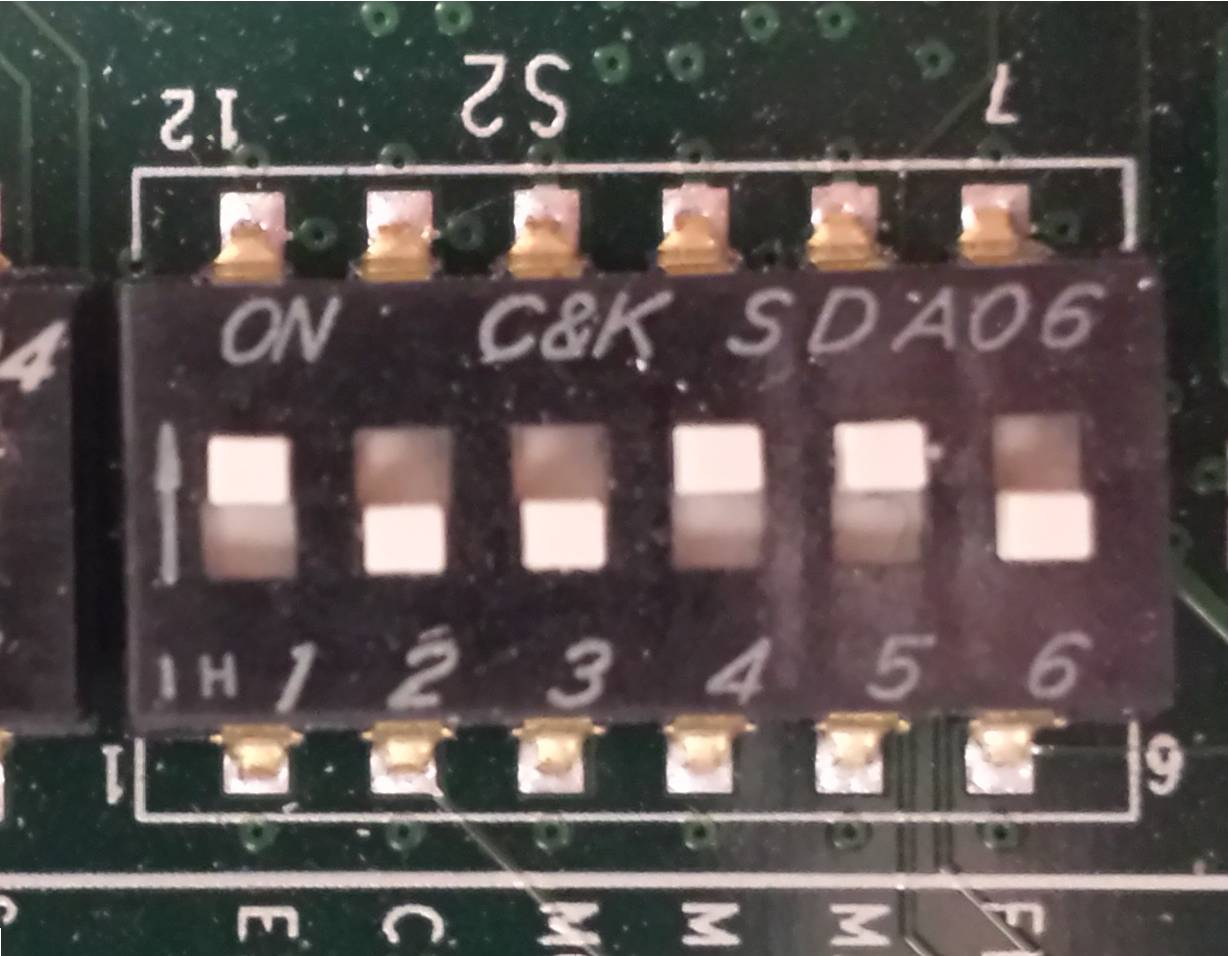
\includegraphics[scale=0.20]{ML605_S2.jpg}\par\smallskip
		The table below contains the expected S2 DIP switch
		settings.\par\smallskip
		\begin{tabular}{|c|c|c|c|c|c|}
		\hline
		\rowcolor{blue}S2.1 & S2.2 & S2.3 & S2.4 & S2.5 & S2.6 \\
		\hline
		on & off & off & on & on & don't care \\
		\hline
		\end{tabular}
	\end{center}\par\bigskip
	\item The J42 configures the board to support 4x PCIe lanes.
	Below is a picture of J42 with a 100mil shunt installed in the
	correct position.
	\begin{center}
		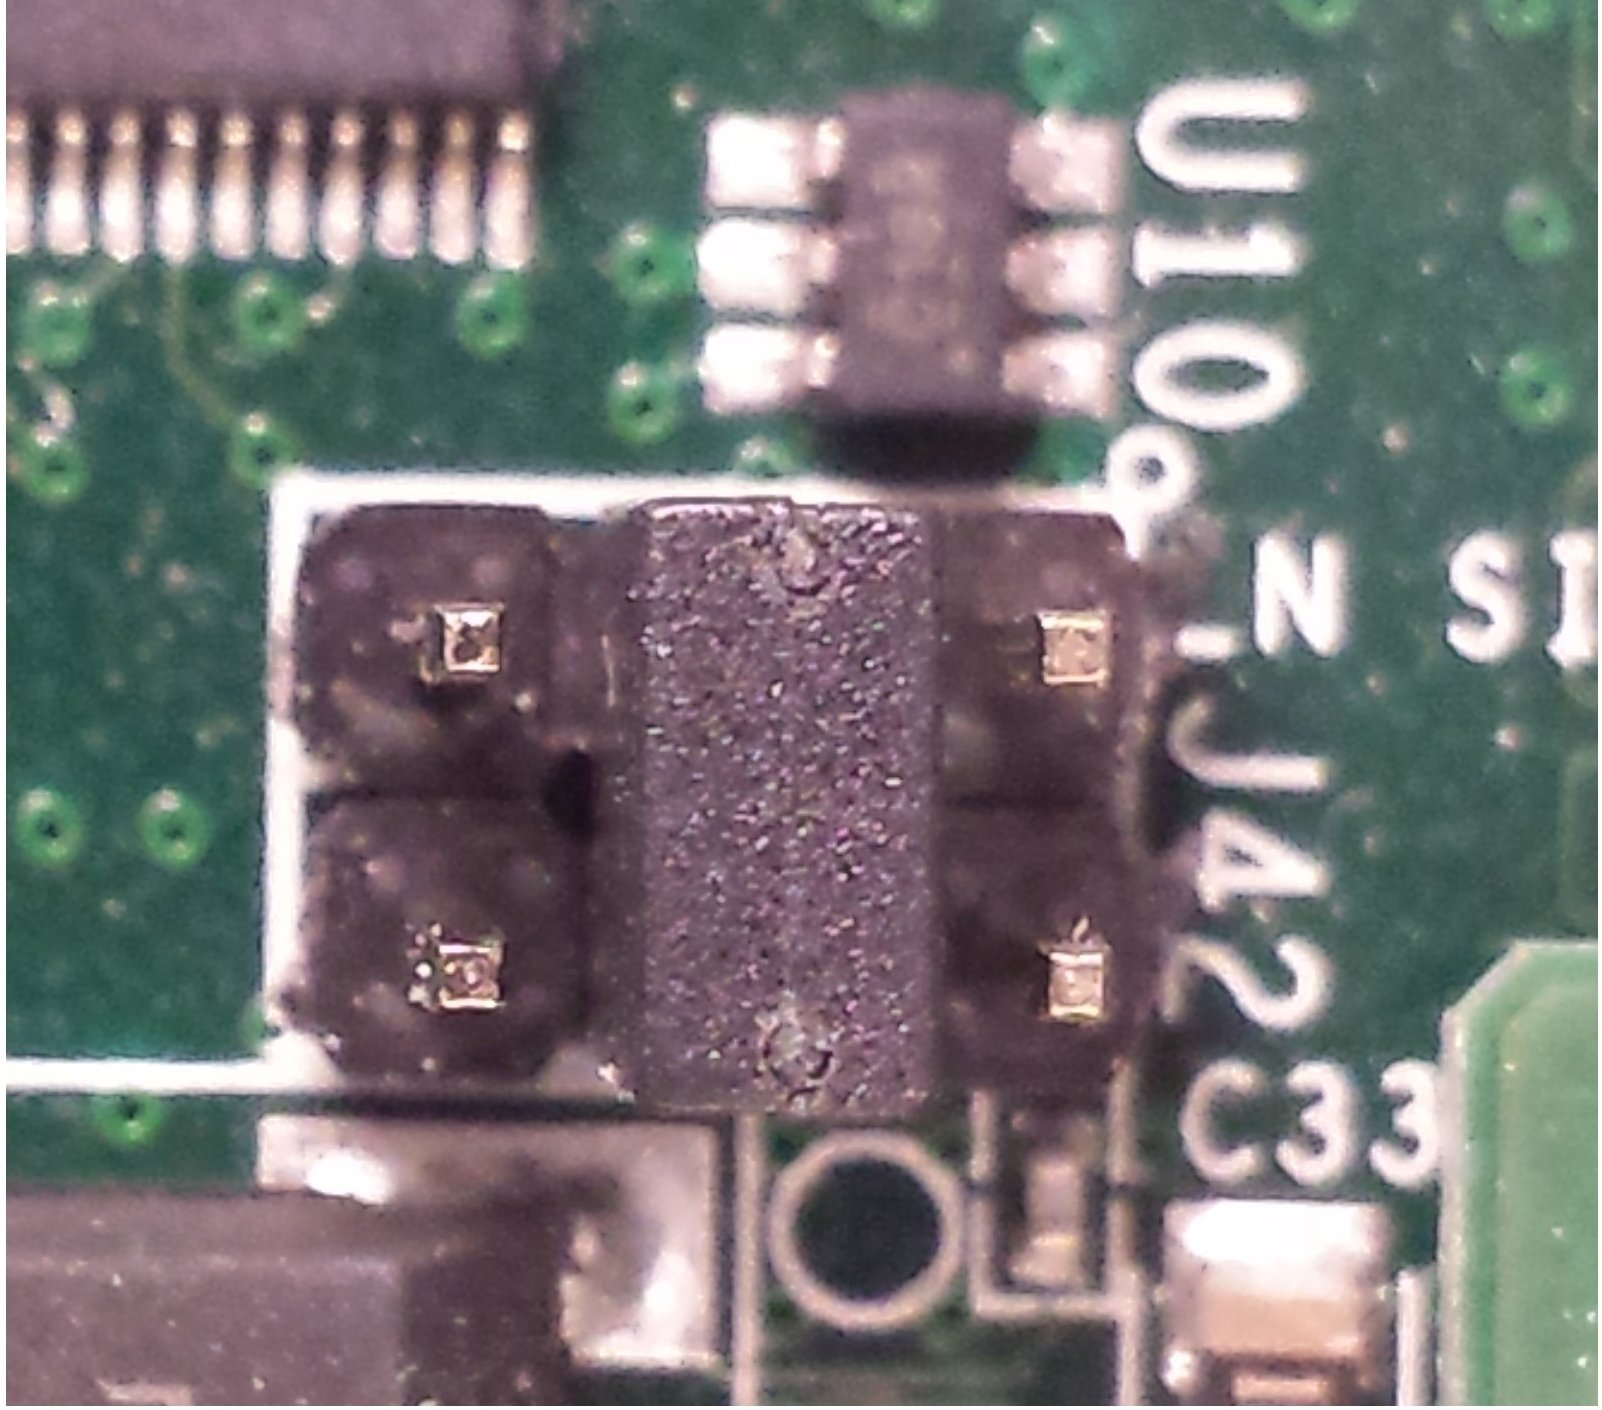
\includegraphics[scale=0.15]{ML605_J42.jpg}\par\bigskip
	\end{center}
\end{enumerate}

\pagebreak
\subsubsection{Install board into OpenCPI development host}
\begin{enumerate}
	\item Power off the development host.
	\item Following anti-static best practices, insert the ML605
	into a compatible PCIe slot.
	\item Attach the USB cable between the ML605 JTAG port and a
	host USB port.
	\item With the AUX power supply unplugged (powered OFF), attach
	the AUX power cable to the ML605 AUX power-in connector.
	\item Power ON the AUX power supply by plugging it an A/C
	outlet. (at this point the development host is still OFF)
	\item Locate the SW2 on the ML605, and switch it to the ON
	position, i.e, slide away from the AUX power-in connector. The
	board will power up, but the development host is not powered on.
	\item Power ON the development host.
\end{enumerate}

\subsubsection{Verify JTAG connection using OpenCPI script}
\begin{enumerate}
\item Open a terminal configured for OpenCPI and run the following script to test the JTAG connection:
	\begin{verbatim}
		$ probeJtag
	\end{verbatim}
	\noindent{\bf Example of the output is shown below:}\smallskip
	\begin{verbatim}
==== Probing for Altera JTAG ports:
Altera directory set by (OCPI_ALTERA_TOOLS_DIR) does not exist.
==== Probing for Xilinx JTAG ports:
Discovered ports are: usb21
Trying port usb21...  ESN is 000013C8121101
Part at position 1 on is xccace
Part at position 2 on is xc6vlx240t.
	\end{verbatim}
For the purposes of this guide, messages related to Altera may be ignored. If the output doesn't look like this, refer Xilinx documentation to ensure the JTAG cable is correctly installed and operational.
\end{enumerate}
\par\smallskip

\subsubsection{Run OpenCPI loadFlash script}
\begin{enumerate}
	\item The loadFlash script is located at
	/opt/opencpi/cdk/scripts. You must pass it a pre-built ML605
	.bitz file generated by OpenCPI and the serial number (in hex)
	of the JTAG cable from probeJtag script above. Programming the
	flash memory with a bitstream takes approximately 10 minutes to
	complete.\par\smallskip
	\noindent{\bf ML605 syntax}\par
	\noindent\shellcmd{
	loadFlash ml605 <OpenCPI Bitstream File>
	<JTAG\_CABLE\_SERIAL\_NUMBER>}
	\par\smallskip

	\noindent{\bf Example command and output:}\smallskip
	\begin{verbatim}
$ loadFlash ml605 hdl/platforms/ml605/testbias_ml605_base.bitz 000013C8121101

Loading the flash memory on the ml605 platform attached to the JTAG pod with ESN 000013C8121101
Loading from file: hdl/platforms/ml605/testbias_ml605_base.bitz
Looking for the Xilinx USB port corresponding to JTAG Pod ESN 000013C8121101.
Discovered ports are: usb21
Trying usb21... ESN is: 000013C8121101
Found ESN 000013C8121101 on usb21, using it.
The bitstream file "hdl/platforms/ml605/testbias_ml605_base.bitz" is compressed. Expanding it.
Bitstream file decompressed into "/tmp/ocpibitstream3100.bit"
Converting "/tmp/ocpibitstream3100.bit" to flash format in
"/tmp/ocpibitstream3100.mcs" using xilinx promgen tool.
Executing command: /opt/Xilinx/14.5/ISE_DS/ISE/bin/lin64/promgen -w -p mcs -c FF
-x xcf128x -data_width 16 -u 00000000 /tmp/ocpibitstream3100.bit
Conversion to flash file format succeeded. Starting flash programming.
This can take a while - 10-15 minutes. Starting at 09:57:27.
real	11m55.080s
user	0m28.494s
sys	0m7.742s
Flash programming is complete. You must power-cycle the system to use it
Use the "ocpihdl search" command after power cycling to confirm success.
	\end{verbatim}
	\item Once programming is complete, power cycle the system:
	\item[i]Power OFF the host
	\item[ii]Power cycle the ML605
	\item[iii]Power ON the host
\end{enumerate}

\subsubsection{Verify that the ML605 is configured with a OpenCPI bitstream}
\begin{enumerate}
	\item Open a terminal window.
	\item Execute the following Linux command to verify the presence of the ML605.
	\begin{verbatim}
$ sudo lspci -vv

03:00.0 RAM memory: Xilinx Corporation Device 4243 (rev 02)
Subsystem: Xilinx Corporation Device 0007
Control: I/O- Mem- BusMaster- SpecCycle- MemWINV- VGASnoop- ParErr- Stepping-
SERR- FastB2B- DisINTx-
Status: Cap+ 66MHz- UDF- FastB2B- ParErr- DEVSEL=fast >TAbort-
<TAbort- <MAbort- >SERR- <PERR- INTx-
	Interrupt: pin A routed to IRQ 11
	Region 0: Memory at e8000000 (32-bit, non-prefetchable) [disabled] [size=64M]
	Region 1: Memory at ec000000 (32-bit, non-prefetchable) [disabled] [size=1M]
	Capabilities: [40] Power Management version 3
		Flags: PMEClk- DSI- D1- D2- AuxCurrent=0mA PME(D0+,D1+,D2+,D3hot+,D3cold-)
		Status: D0 NoSoftRst+ PME-Enable- DSel=0 DScale=0 PME-
	Capabilities: [48] MSI: Enable- Count=1/1 Maskable- 64bit+
		Address: 0000000000000000  Data: 0000
	Capabilities: [60] Express (v2) Endpoint, MSI 01
		DevCap:	MaxPayload 512 bytes, PhantFunc 0, Latency L0s <64ns, L1 unlimited
			ExtTag- AttnBtn- AttnInd- PwrInd- RBE+ FLReset-
		DevCtl:	Report errors: Correctable- Non-Fatal- Fatal- Unsupported-
			RlxdOrd- ExtTag- PhantFunc- AuxPwr- NoSnoop+
			MaxPayload 256 bytes, MaxReadReq 256 bytes
		DevSta:	CorrErr- UncorrErr- FatalErr- UnsuppReq- AuxPwr- TransPend-
		LnkCap:	Port \#0, Speed 5GT/s, Width x4, ASPM L0s, Latency L0 unlimited, L1 unlimited
			ClockPM- Surprise- LLActRep- BwNot-
		LnkCtl:	ASPM Disabled; RCB 64 bytes Disabled- Retrain- CommClk-
			ExtSynch- ClockPM- AutWidDis- BWInt- AutBWInt-
		LnkSta:	Speed 5GT/s, Width x4, TrErr- Train- SlotClk- DLActive- BWMgmt- ABWMgmt-
		DevCap2: Completion Timeout: Range B, TimeoutDis-, LTR-, OBFF Not Supported
		DevCtl2: Completion Timeout: 50us to 50ms, TimeoutDis-, LTR-, OBFF Disabled
		LnkCtl2: Target Link Speed: 5GT/s, EnterCompliance- SpeedDis-
			 Transmit Margin: Normal Operating Range, EnterModifiedCompliance- ComplianceSOS-
			 Compliance De-emphasis: -6dB
		LnkSta2: Current De-emphasis Level: -3.5dB, EqualizationComplete-, EqualizationPhase1-
			 EqualizationPhase2-, EqualizationPhase3-, LinkEqualizationRequest-
	Capabilities: [100 v1] Device Serial Number 00-00-00-01-01-00-0a-35
	Kernel modules: windrvr6
	\end{verbatim}
	\item In the terminal window configured for OpenCPI, execute the
	OpenCPI utility that executes Xilinx iMPACT to scan JTAG for
	devices:\smallskip
	\begin{verbatim}
$ probeJtag

==== Probing for Altera JTAG ports:
Altera directory (set by OCPI_ALTERA_TOOLS_DIR) does not exist.
==== Probing for Xilinx JTAG ports:
Discovered ports are: usb21
Trying port usb21...  ESN is 000013C8121101
Part at position 1 on is xccace
Part at position 2 on is xc6vlx240t
	\end{verbatim}\par\smallskip
	\item Load the OpenCPI driver (requires sudo privileges):\smallskip
	\begin{verbatim}
		$ ocpidriver load
	\end{verbatim}
	\item Execute an OpenCPI utility\smallskip
	\begin{verbatim}
$ ocpihdl search
OpenCPI HDL device found: 'PCI:0000:03:00.0': bitstream date Fri Jun 26 15:14:21 2015,
platform "ml605", part "xc6vlx240t", UUID 8cd0a91e-1c37-11e5-8b5f-f30e2f82978a
	\end{verbatim}
	\item Perform a container check using ocpirun -C. The result
	should look like this:\smallskip
	\begin{verbatim}
$ ocpirun -C
Available containers:
 #  Model Platform    OS     OS Version  Arch   Name
 0  rcc   centos7     linux  c7          x86_64 rcc0
 1  hdl   ml605                                 PCI:0000:03:00.0
  	\end{verbatim}
\end{enumerate}

\subsubsection{Modification of /opt/opencpi/system.xml}
When multiple boards from same vendor are installed, and thus more than one JTAG USB, the OpenCPI load function (either explicit in ``ocpihdl load'' or implicit in 'ocpirun' needs to know which JTAG USB to use. The '/opt/opencpi/system.xml' file is used to map the PCI:* with JTAG USB serial number information. An example is shown below:
	\begin{verbatim}
<opencpi>
    <container>
        <hdl>
        <device name="0000:03:00.0" esn="000013C8121101"/>
        <device name="0000:08:00.0" esn="000013C84C2F01"/>
        </hdl>
    </container>
</opencpi>
	\end{verbatim}
Perform a container check using \textit{ocpirun -C}. The result should look like this:
	\begin{verbatim}
$ ocpirun -C
Available containers:
 #  Model Platform    OS       OS Version  Arch   Name
 0  rcc   centos7     linux    c7          x86_64 rcc0
 1  hdl   ml605                                   PCI:0000:08:00.0
 2  hdl   ml605                                   PCI:0000:03:00.0
	\end{verbatim}

\end{document}
